\documentclass[]{report}

\usepackage{graphicx}
\usepackage{float}
\usepackage{enumitem}
\usepackage{tabularx}
\usepackage{hyperref}
\usepackage[normalem]{ulem}
\usepackage{listings}
\usepackage[most]{tcolorbox}

\definecolor{commentsColor}{rgb}{0.497495, 0.497587, 0.497464}
\definecolor{keywordsColor}{rgb}{0.000000, 0.000000, 0.635294}
\definecolor{stringColor}{rgb}{0.558215, 0.000000, 0.135316}

\lstset{
	columns=flexible,
	breaklines=true,
	backgroundcolor=\color{white},   % choose the background color
	basicstyle=\small\ttfamily,        % the size of the fonts that are used for the code
	breakatwhitespace=false,         % sets if automatic breaks should only happen at whitespace
	breaklines=true,                 % sets automatic line breaking
	captionpos=b,                    % sets the caption-position to bottom
	commentstyle=\color{commentsColor}\textit,    % comment style
	deletekeywords={},            % if you want to delete keywords from the given language
	escapeinside={\%*}{*)},          % if you want to add LaTeX within your code
	extendedchars=true,              % lets you use non-ASCII characters; for 8-bits encodings only, does not work with UTF-8
	%frame=tb,	                   	   % adds a frame around the code
	keepspaces=true,                 % keeps spaces in text, useful for keeping indentation of code (possibly needs columns=flexible)
	keywordstyle=\color{keywordsColor}\bfseries,       % keyword style
	language=C++,                 % the language of the code (can be overrided per snippet)
	otherkeywords={rank\_t, customerID\_t, distance\_t, fitness\_t},           % if you want to add more keywords to the set
	numbers=left,                    % where to put the line-numbers; possible values are (none, left, right)
	numbersep=5pt,                   % how far the line-numbers are from the code
	numberstyle=\tiny\color{commentsColor}, % the style that is used for the line-numbers
	rulecolor=\color{black},         % if not set, the frame-color may be changed on line-breaks within not-black text (e.g. comments (green here))
	showspaces=false,                % show spaces everywhere adding particular underscores; it overrides 'showstringspaces'
	keepspaces=true,
	showstringspaces=false,          % underline spaces within strings only
	showtabs=false,                  % show tabs within strings adding particular underscores
	stepnumber=1,                    % the step between two line-numbers. If it's 1, each line will be numbered
	stringstyle=\color{stringColor}, % string literal style
	tabsize=4,	                   % sets default tabsize to 2 spaces
	title=\lstname,                  % show the filename of files included with \lstinputlisting; also try caption instead of title
	columns=fixed                    % Using fixed column width (for e.g. nice alignment)
}
\lstMakeShortInline|

\newtcolorbox{answerbox}[2][]{%
	attach boxed title to top center
	= {yshift=-8pt},
	colback      = black!5!white,
	colframe     = black!75!black,
	fonttitle    = \bfseries,
	colbacktitle = gray!85!black,
	title        = #2,#1,
	enhanced,
}

\lstset{
	basicstyle=\small\ttfamily,
	columns=flexible,
	breaklines=true
}

\usepackage{float}

\renewcommand{\thesection}{\arabic{section}}

% Title Page
\title{\textbf{COSC 4P82 Assignment 1}}
\author{\textbf{Brett Terpstra}\\
	bt19ex@brocku.ca - 692021}

\begin{document}
\maketitle
\tableofcontents

\section{Introduction}

\section{Symbolic regression}
\subsection{Introduction}
\subsection{Parameter Table}
\begin{center}
\begin{tabularx}{0.8\textwidth}{ | >{\centering\arraybackslash}X | >{\centering\arraybackslash}X | }
	\hline
	Parameter & Value \\ [0.25ex]
	\hline\hline
	Runs & 10 \\
	\hline
	Population Size & 5000 \\
	\hline
	Generations & 50 \\
	\hline
	Training Set & N/A \\
	\hline
	Testing Set & N/A \\
	\hline
	Crossover Operator & Subtree Crossover\\
	\hline
	Mutation Operator & Grow Tree, Max Depth 4 \\
	\hline
	Crossover Rate & 0.9 or 1.0* \\
	\hline
	Mutation Rate & 0.1 or 1.0* \\
	\hline
	Elitism & Best 2 or 0 individuals Survive* \\
	\hline
	Selection & Fitness Proportionate \\
	\hline
	Function Set & *, /, +, -, exp, log, sin, cos \\
	\hline
	Terminal Set & X, Ephemeral Value \\
	\hline
	Tree Initialization & Half and Half, Max Depth 2-6 \\
	\hline
	Max Tree Depth & 17 \\
	\hline
	Raw Fitness & See Fitness Evaluation \\
	\hline
	Standardized Fitness & = Raw Fitness \\
	\hline
\end{tabularx}
\end{center}
*4 Tests were run, 0.9 crossover, 0.9 mutation with 0 elitism and 2 elitism, and 1.0 crossover, 1.0 mutation with 0 elitism and 2 elitism.
\subsection{Fitness Evaluation}
Fitness is evaluated by taking the absolute value of the predicted y value minus the actual y value. 
If the difference is less than a user provided (default 1.e15) value cutoff it is added to the fitness value. If the difference value is less than the float epsilon value (\~= 0) the number of hits is incremented. Lower fitness values are preferred.  
\subsection{Fitness Plots}
\begin{figure}[H]
	\centering
	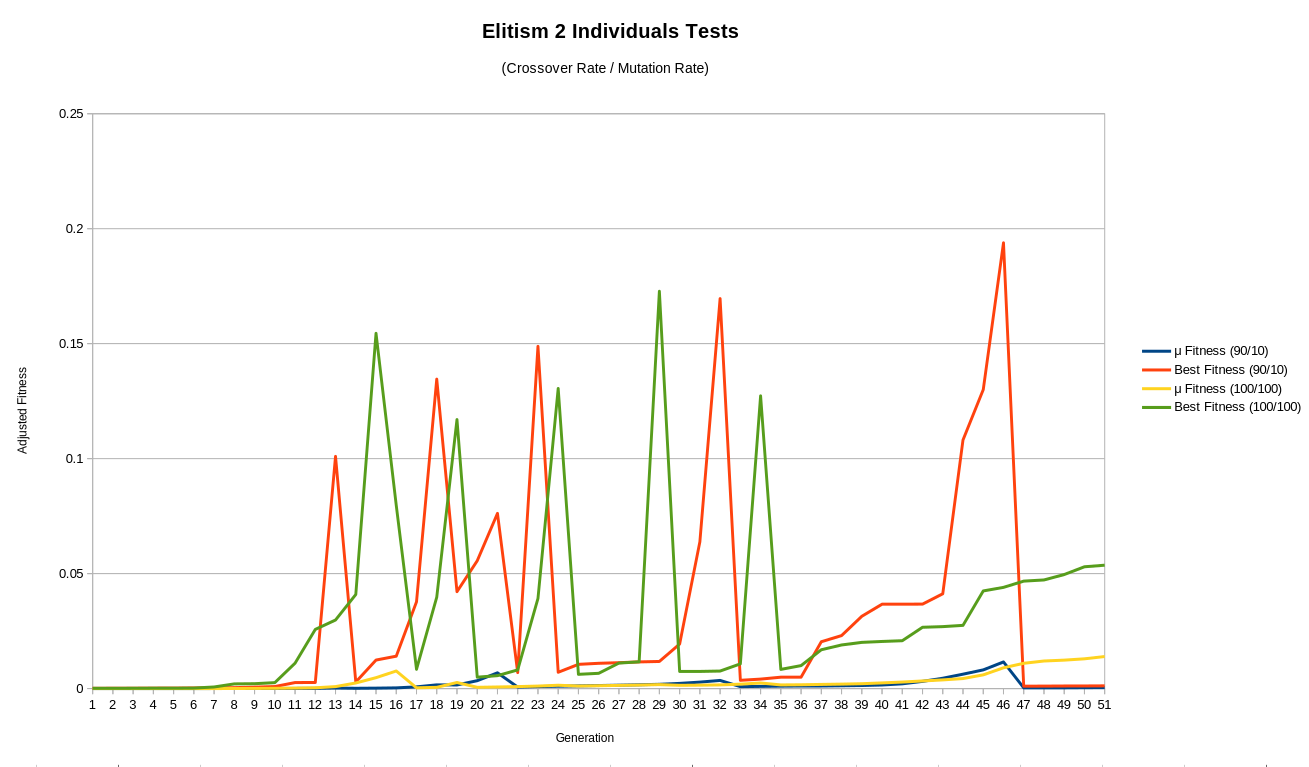
\includegraphics[width=1.0\linewidth]{fp5}
	\caption{2 Elites, 10 Runs Averaged}
	\label{fig:fp4}
\end{figure}
\begin{figure}[H]
	\centering
	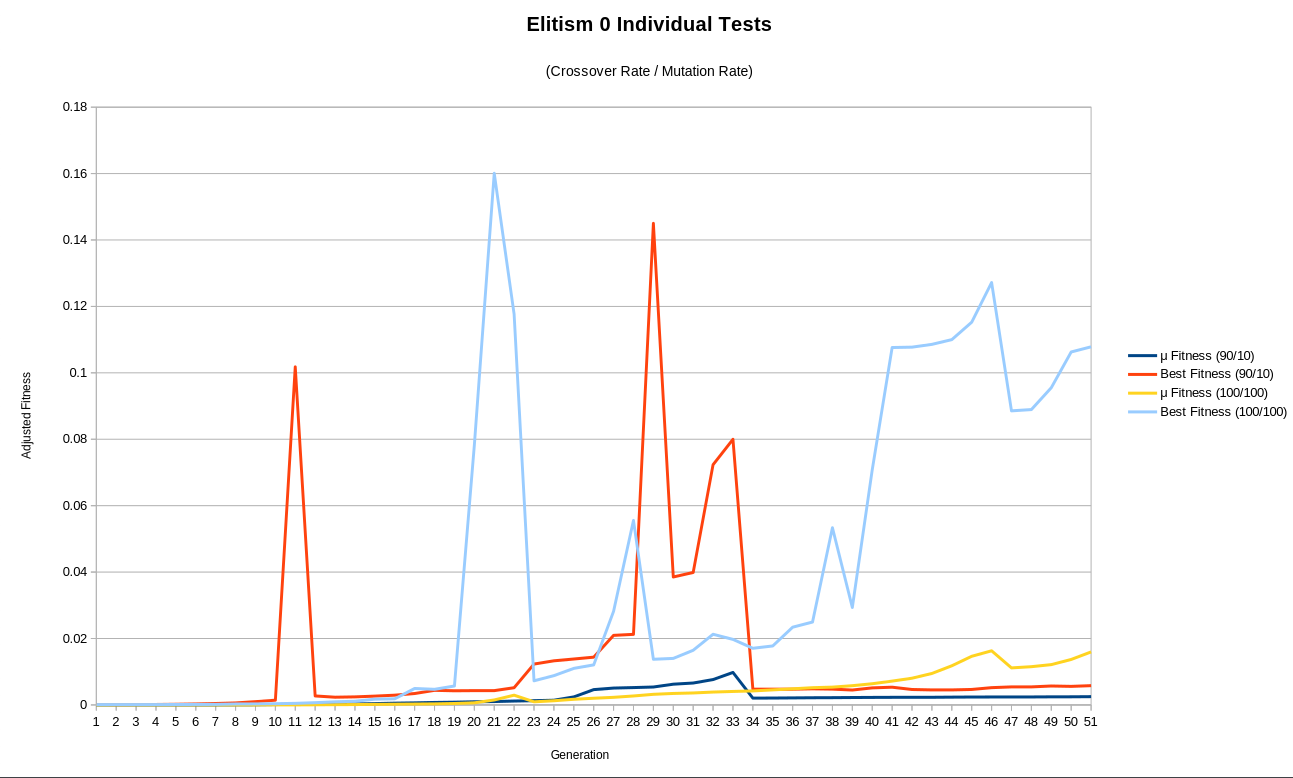
\includegraphics[width=1.0\linewidth]{fp3}
	\caption[]{0 Elites, 10 Runs Averaged}
	\label{fig:fp2}
\end{figure}
\subsection{Analysis and Conclusion}
The best average fitness of all the tests was 0.19384 using 0.9 crossover and 0.1 mutation. 

\section{Rice Classification}
\subsection{Introduction}
\subsection{Parameter Table}
\begin{center}
	\begin{tabularx}{0.8\textwidth}{ | >{\centering\arraybackslash}X | >{\centering\arraybackslash}X | }
		\hline
		Parameter & Value \\ [0.25ex]
		\hline\hline
		Runs & 10 \\
		\hline
		Population Size & 5000 \\
		\hline
		Generations & 51 \\
		\hline
		Training Set & Rice Classification (Cammeo and Osmancik) \\
		\hline
		Testing Set & Rice Classification (Cammeo and Osmancik) \\
		\hline
		Crossover Operator & Subtree Crossover\\
		\hline
		Mutation Operator & Grow Tree, Max Depth 4 \\
		\hline
		Crossover Rate & 0.9 or 0.9* \\
		\hline
		Mutation Rate & 0.1 or 0.9* \\
		\hline
		Elitism & Best 2 individuals Survive \\
		\hline
		Selection & Fitness Proportionate \\
		\hline
		Function Set & *, /, +, -, exp, log \\
		\hline
		Terminal Set & area, perimeter, major, minor, eccentricity, convex, extent, Ephemeral Value \\
		\hline
		Tree Initialization & Half and Half, Max Depth 2-6 \\
		\hline
		Max Tree Depth & 17 \\
		\hline
		Raw Fitness & See Fitness Evaluation \\
		\hline
		Standardized Fitness & = Raw Fitness \\
		\hline
	\end{tabularx}
\end{center}
\subsection{Fitness Evaluation}
Tested on the input terminal values the GP produces a positive or negative value which is interpreted as either Cammeo (+) or Osmancik (-). Raw fitness is equal to the number of hits which is the number of correct identifications. The adjusted fitness is then calculated and subtracted from 1 in order to invert and produce the required lowest fitness better.
\subsection{Fitness Plots}
\begin{figure}[H]
	\centering
	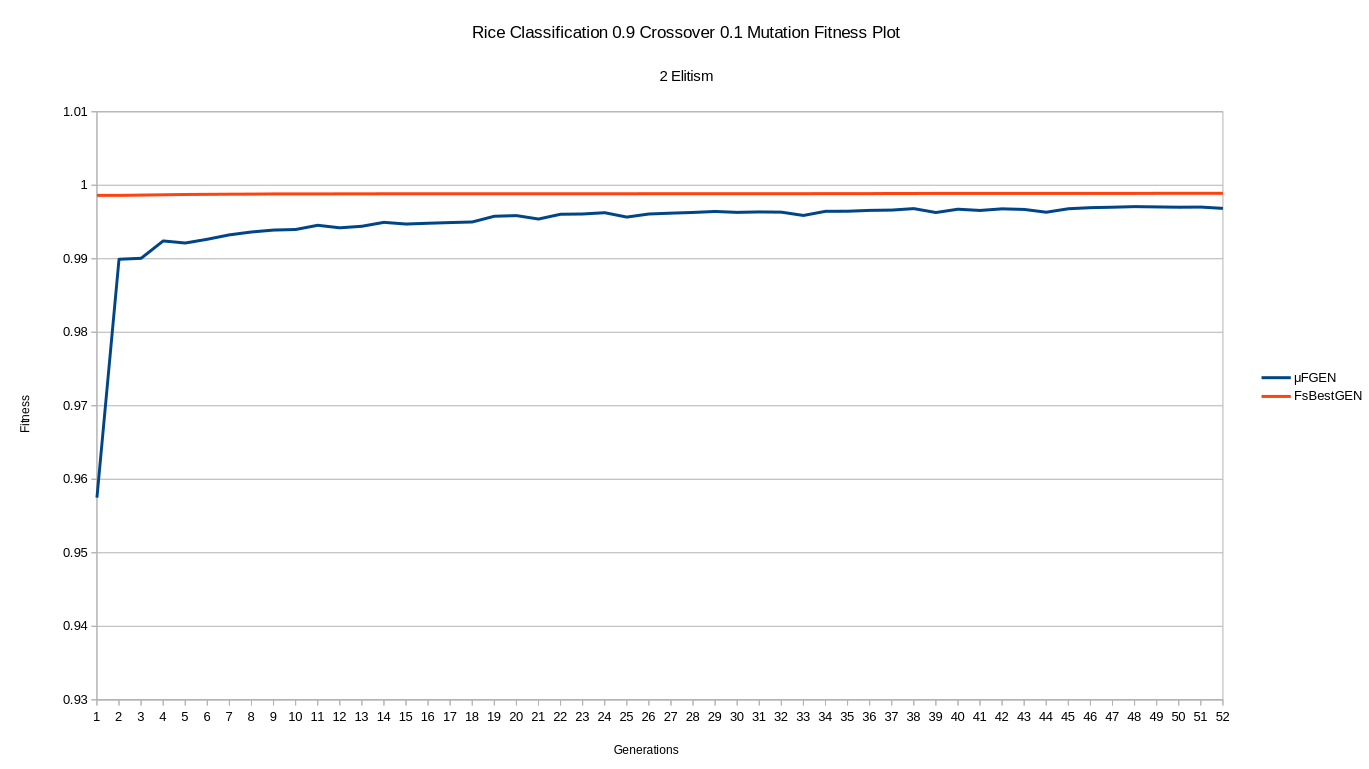
\includegraphics[width=1.0\linewidth]{fp6}
	\caption{2 Elites, 10 Runs Averaged}
	\label{fig:fp6}
\end{figure}
\begin{figure}[H]
	\centering
	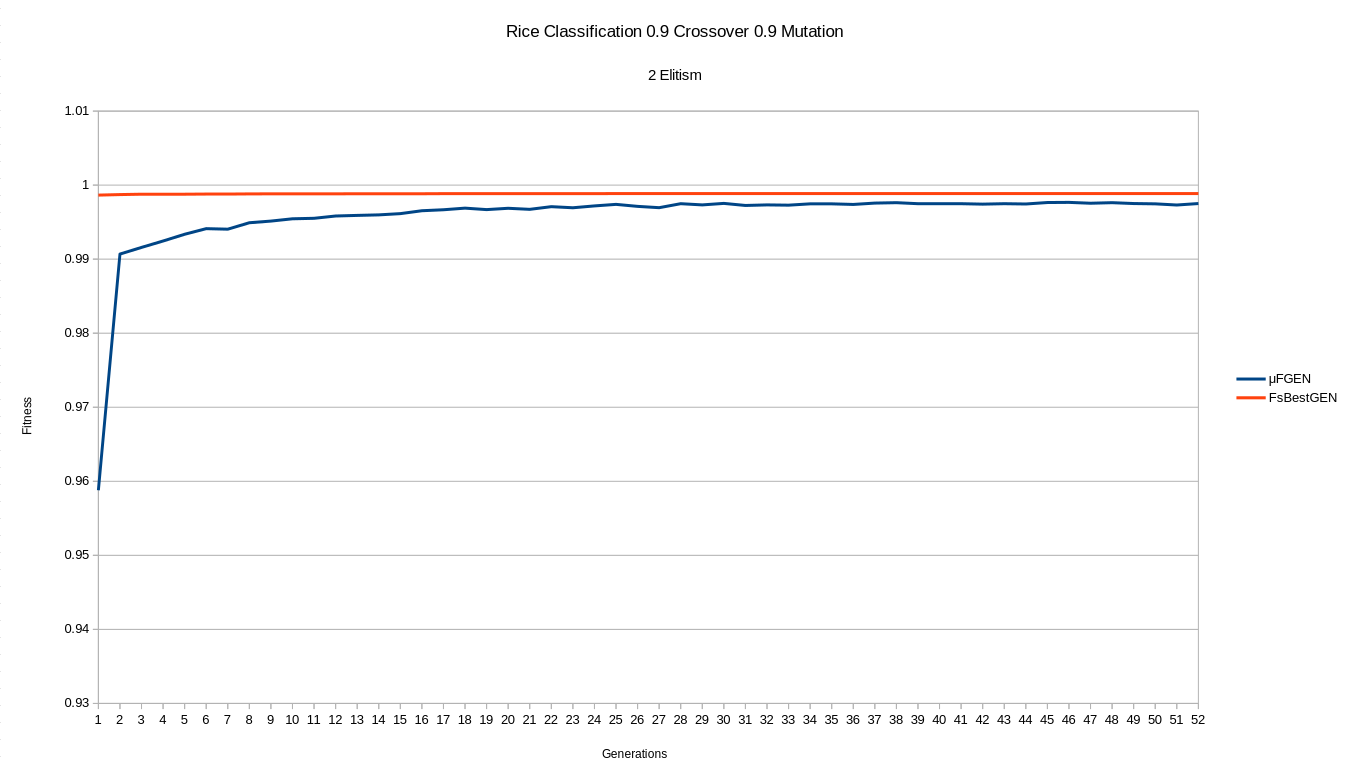
\includegraphics[width=1.0\linewidth]{fp7}
	\caption{2 Elites, 10 Runs Averaged}
	\label{fig:fp7}
\end{figure}


\subsection{Confusion Matrix}

\begin{figure}[H]
	\centering
	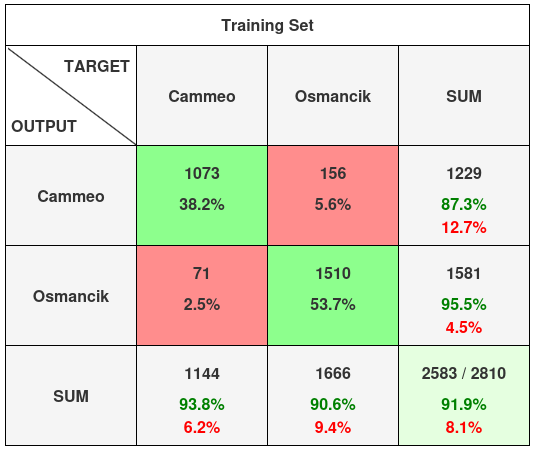
\includegraphics[width=1.0\linewidth]{fp10}
	\caption{0.9 Crossover 0.1 Mutation 2 Elites Best Program Results}
	\label{fig:fp10}
\end{figure}

\begin{figure}[H]
	\centering
	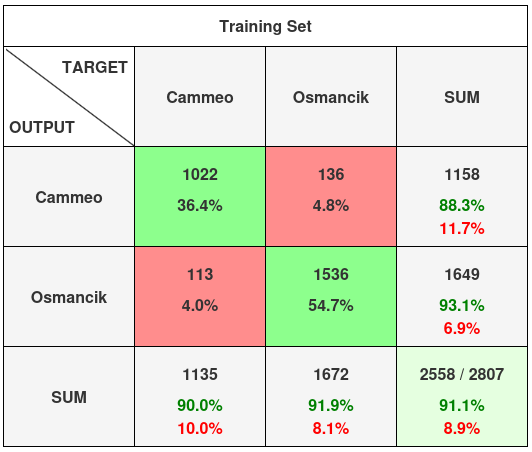
\includegraphics[width=1.0\linewidth]{fp11}
	\caption{0.9 Crossover 0.1 Mutation 2 Elites 10 Run Average Results}
	\label{fig:fp11}
\end{figure}



\begin{figure}[H]
	\centering
	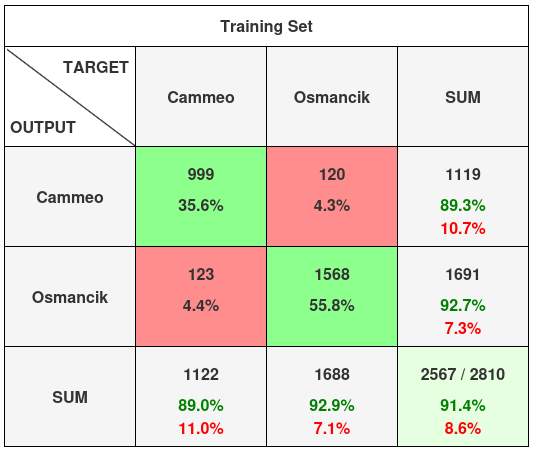
\includegraphics[width=1.0\linewidth]{fp12}
	\caption{0.9 Crossover 0.9 Mutation 2 Elites Best Program Results}
	\label{fig:fp8}
\end{figure}
\begin{figure}[H]
	\centering
	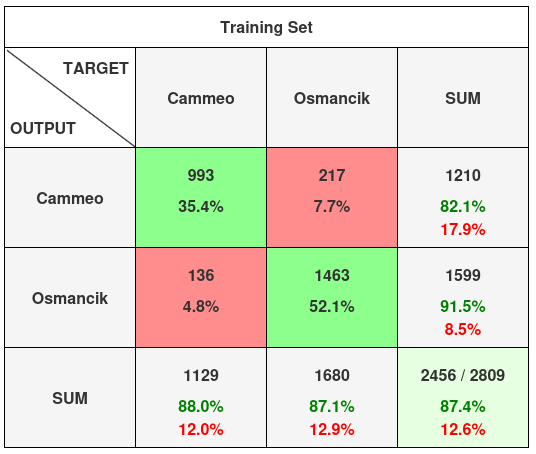
\includegraphics[width=1.0\linewidth]{fp13}
	\caption{0.9 Crossover 0.9 Mutation 2 Elites 10 Run Average Results}
	\label{fig:fp9}
\end{figure}

\subsection{Analysis and Conclusion}
The best results found was a correct classification rate of 91.9\%. On average the 0.9 crossover with 0.1 mutation produced the best results with the 0.9/0.9 best result almost being equal.


\section{Compiling / Executing}
This assignment was made for linux using GCC 13.2.0, however any C++17 compliant compiler should work. 
The minimum GCC version appears to be 8.5, meaning this assignment can be built on sandcastle.
\begin{lstlisting}
	cd your_path_to_this_source/
	mkdir build
	cd build
	cmake ../
	make -j 32
\end{lstlisting}
The actual assignment executable is called |Assignment_1| while the automatic run system is called |Assignment_1_RUNNER|. |Assignment_1_RUNNER| has a help menu with options but the defaults will work assuming you run from the build directory and are using part b only. If you want to build for Part A run |cmake -DPART_B=OFF| and run |Assignment_1_RUNNER| with |-b|

\section{Conclusion}
I made a few changes to lilgp, mostly memory fixes along with elitism with a number of individuals instead of a proportion. There appear to be some kind of issue in the GP, of which won't matter as assignment two will likely use my own gp system. I might look into it, but I was not aware there was an issue until compiling the stats here. My results have been generally positive, however, I did notice in the course of collecting data that at some point the Part A results stopped being consistently good however part B results have remained unchanged. Might have happened when I changed my custom random number seeder to not produce div by zero errors during testing. Could be anything. I don't like writing reports and have procrastinated on writing and instead have spent the last couple of weeks messing around with the GP. Fun fact a bunch of additions to my standard lib were made for this assignment. Next time will be better hopefully

\section{References}
Next assignment these will be proper. Latex is being annoying to setup for bib.\\\\
https://archive.ics.uci.edu/dataset/545/rice+cammeo+and+osmancik\\
http://garage.cse.msu.edu/software/lil-gp/

\end{document}          
